\clearpage
\begin{figure}[t!]
  \begin{center}
    \subfigure[Hadronic sample (linear scale)]{
      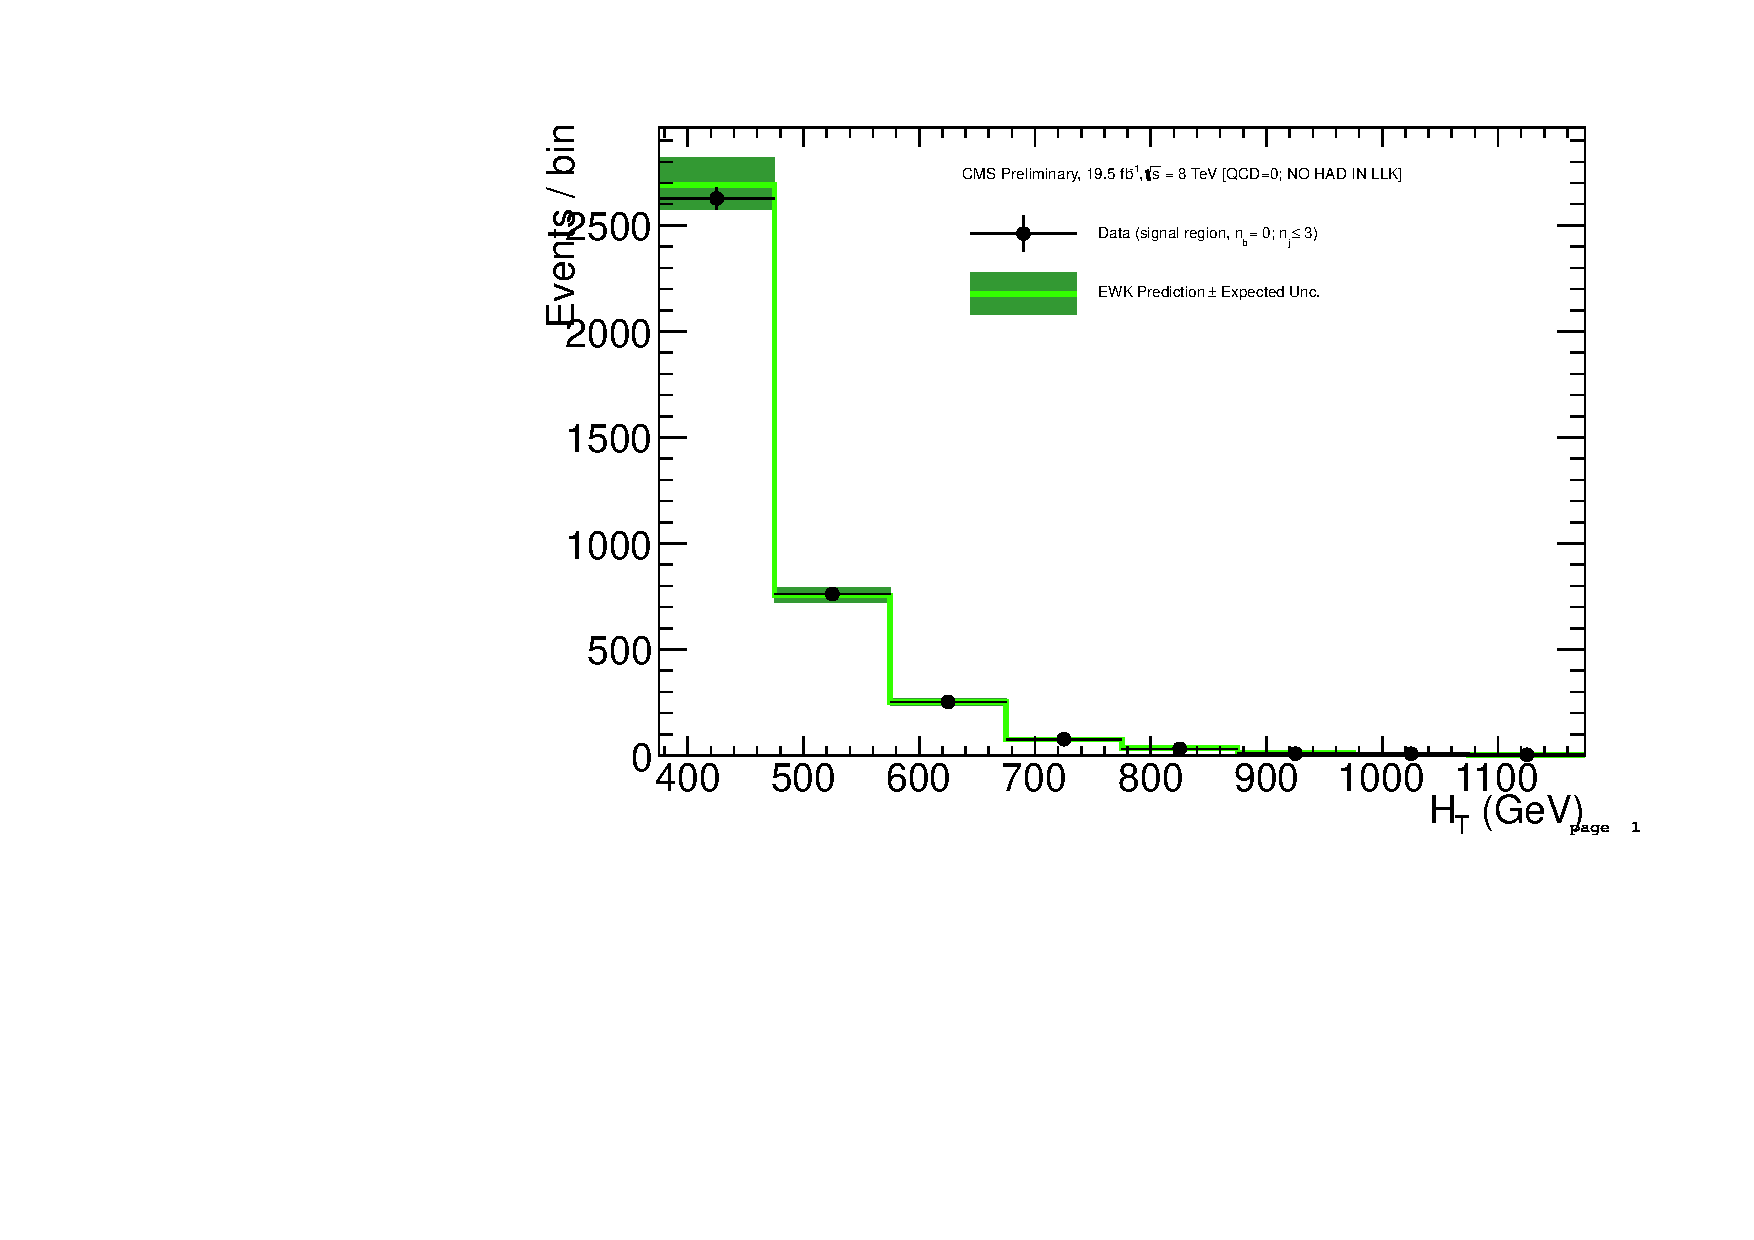
\includegraphics[width=0.45\textwidth,page=1]{figures/fit/v21/bestFit_2012pf_RQcdZero_fZinvAll_0b_le3j-1p_smOnly}
    } 
    \subfigure[Hadronic sample (logarithmic scale)]{
      \includegraphics[width=0.45\textwidth,page=2]{figures/fit/v21/bestFit_2012pf_RQcdZero_fZinvAll_0b_le3j-1p_smOnly}
    } \\
    \subfigure[$\mu$ + jets sample]{
      \includegraphics[width=0.45\textwidth,page=4]{figures/fit/v21/bestFit_2012pf_RQcdZero_fZinvAll_0b_le3j-1p_smOnly}
    } 
    \subfigure[$\gamma$ + jets sample]{
      \includegraphics[width=0.45\textwidth,page=6]{figures/fit/v21/bestFit_2012pf_RQcdZero_fZinvAll_0b_le3j-1p_smOnly}
    } 
    \caption{\label{fig:best-fit-control-only-le3j0b} Comparison of the
      \scalht-binned observed data yields and SM expectations
      when requiring \njetlow and $\nb = 0$ for the (a-b) hadronic,
      (c) \mj, (d) \mmj and (e) \gj samples, as determined by a
      simultaneous fit to the data control samples only. The observed
      event yields in data (black dots) and the expectations and their
      uncertainties (dark green solid line with light green bands), as
      determined by the simultaneous fit, are shown. }
%      For illustrative purposes only, the signal expectations (pink
%      dashed line) for the model \texttt{T2cc} with $m_{\sq} =
%      250\GeV$ and $m_{\text{LSP}} = 240\GeV$ are stacked on top of
%      the SM expectations.}
  \end{center}
\end{figure}

\clearpage
\begin{figure}[t!]
  \begin{center}
    \subfigure[Hadronic sample (linear scale)]{
      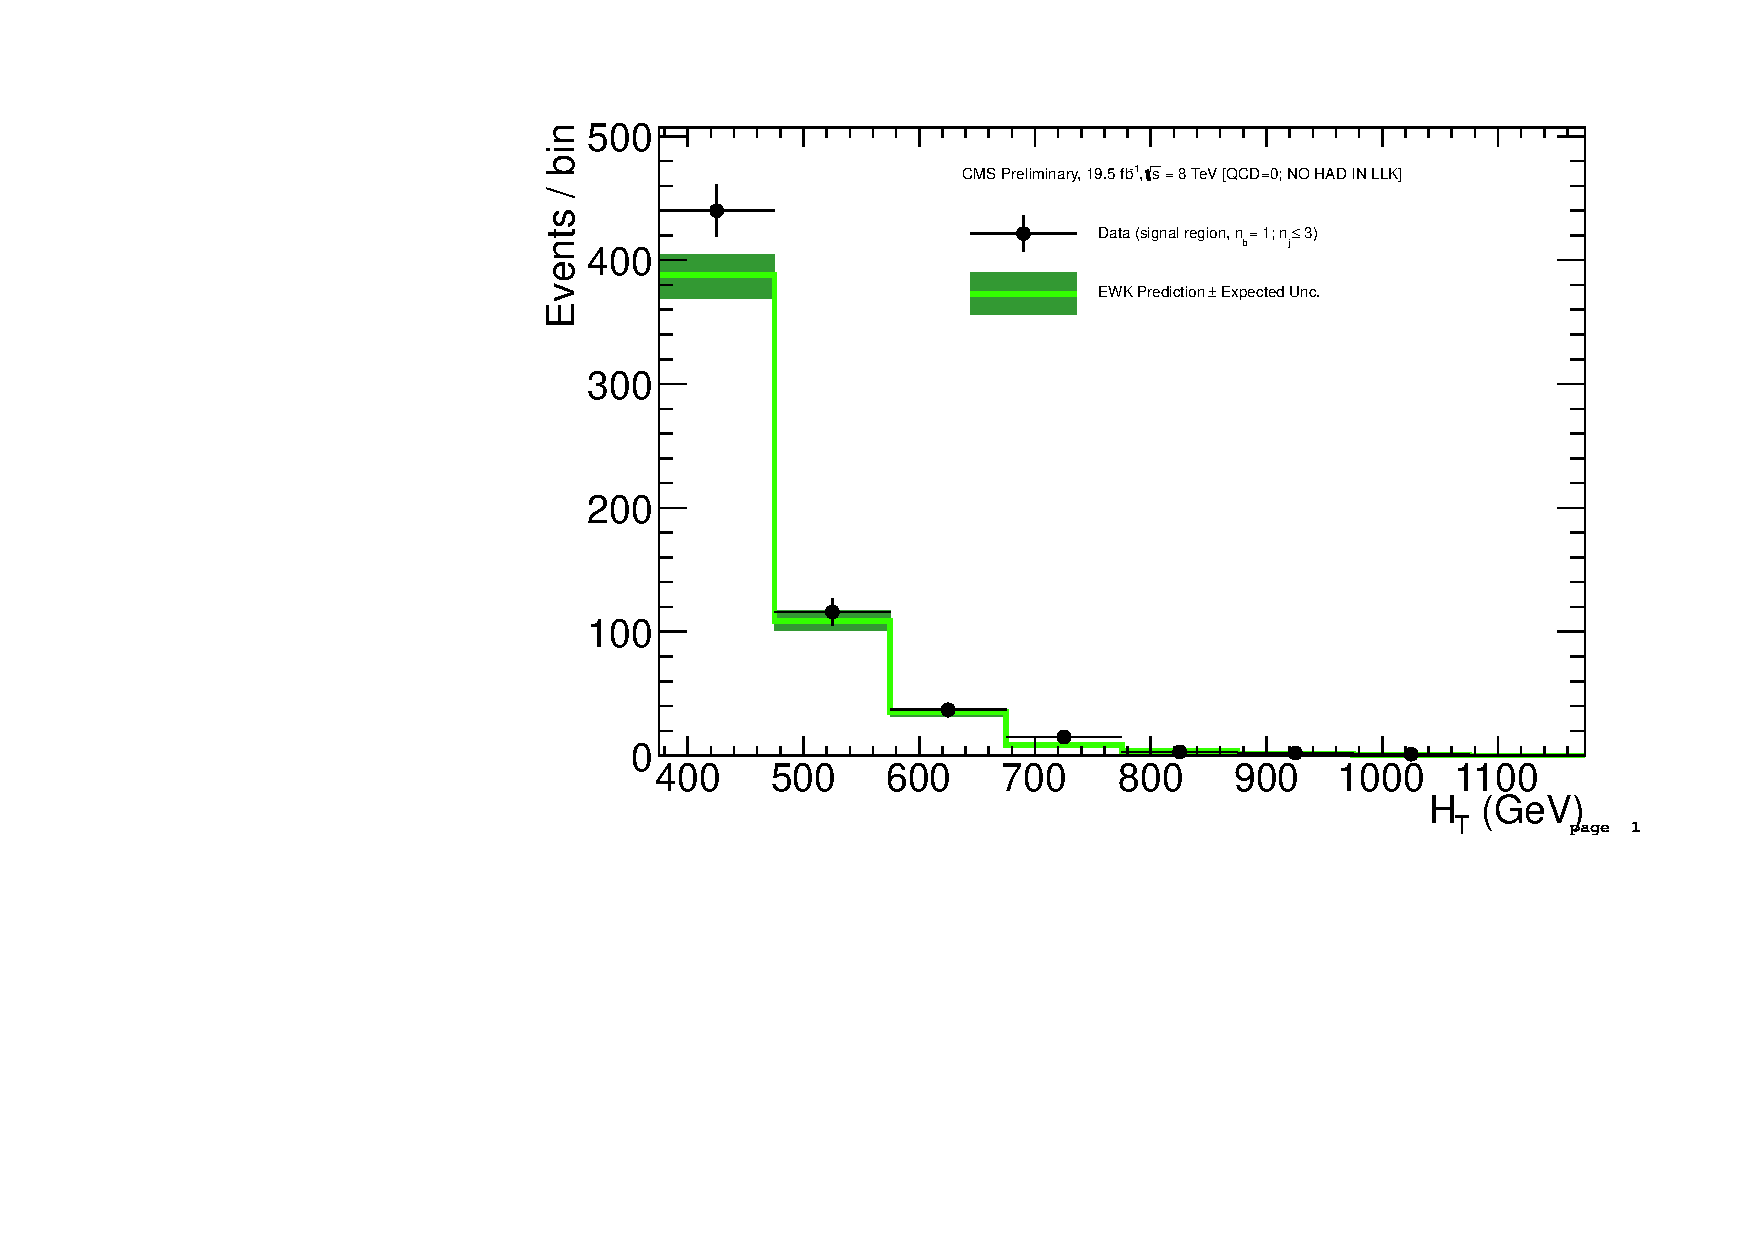
\includegraphics[width=0.45\textwidth,page=1]{figures/fit/v21/bestFit_2012pf_RQcdZero_fZinvAll_1b_le3j-1p_smOnly}
    } 
    \subfigure[Hadronic sample (logarithmic scale)]{
      \includegraphics[width=0.45\textwidth,page=2]{figures/fit/v21/bestFit_2012pf_RQcdZero_fZinvAll_1b_le3j-1p_smOnly}
    } \\
    \subfigure[$\mu$ + jets sample]{
      \includegraphics[width=0.45\textwidth,page=4]{figures/fit/v21/bestFit_2012pf_RQcdZero_fZinvAll_1b_le3j-1p_smOnly}
    } 
    \subfigure[$\gamma$ + jets sample]{
      \includegraphics[width=0.45\textwidth,page=6]{figures/fit/v21/bestFit_2012pf_RQcdZero_fZinvAll_1b_le3j-1p_smOnly}
    } 
    \caption{\label{fig:best-fit-control-only-le3j1b} Comparison of the
      \scalht-binned observed data yields and SM expectations when
      requiring \njetlow and $\nb = 1$ for the (a-b) hadronic, (c)
      \mj, (d) \mmj and (e) \gj samples, as determined by a
      simultaneous fit to the data control samples only. The observed
      event yields in data (black dots) and the expectations and their
      uncertainties (dark green solid line with light green bands), as
      determined by the simultaneous fit, are shown. }
%      For illustrative purposes only, the signal expectations (pink
%      dashed line) for the model \texttt{T2cc} with $m_{\sq} =
%      250\GeV$ and $m_{\text{LSP}} = 170\GeV$ are stacked on top of
%      the SM expectations.}
  \end{center}
\end{figure}

\clearpage
\begin{figure}[t!]
  \begin{center}
    \subfigure[Hadronic sample (linear scale)]{
      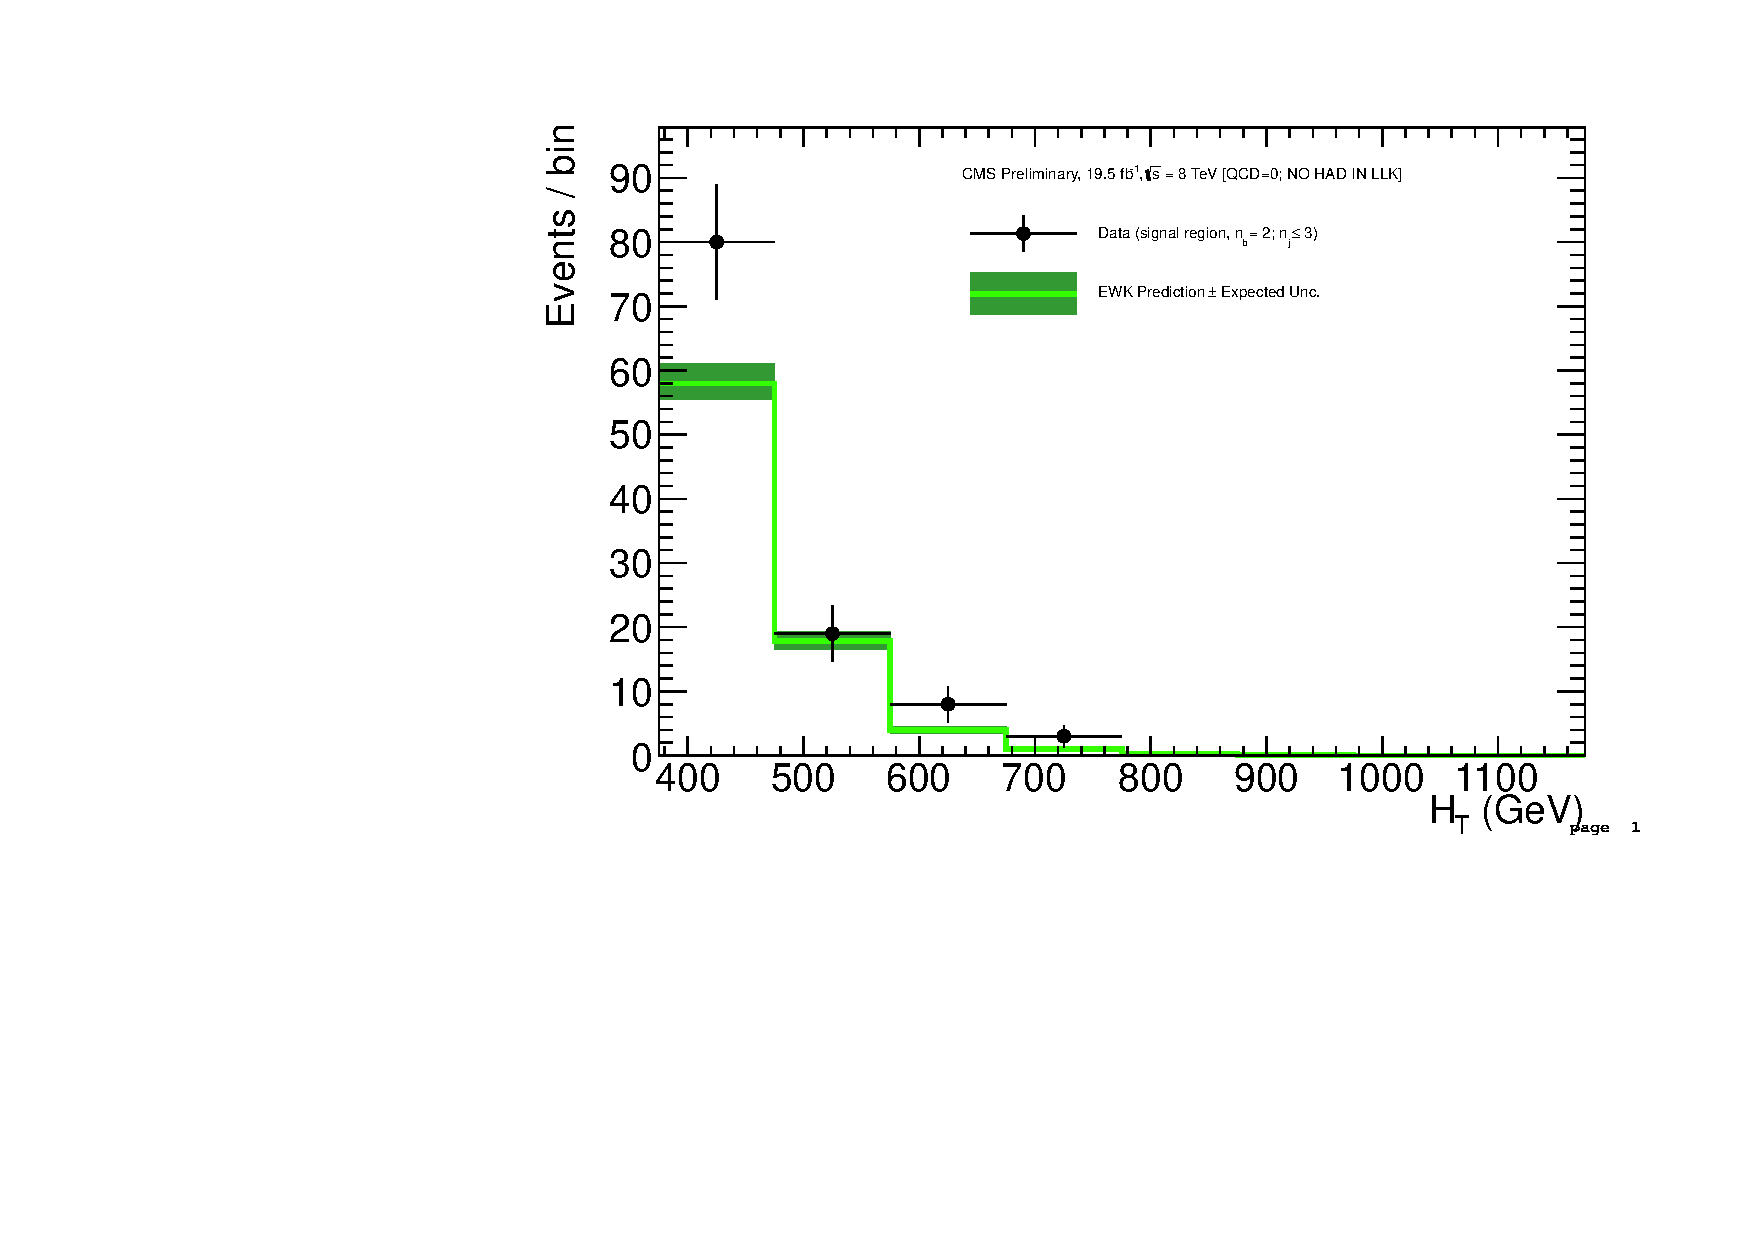
\includegraphics[width=0.45\textwidth,page=1]{figures/fit/v21/bestFit_2012pf_RQcdZero_fZinvAll_2b_le3j-1_smOnly}
    } 
    \subfigure[Hadronic sample (logarithmic scale)]{
      \includegraphics[width=0.45\textwidth,page=2]{figures/fit/v21/bestFit_2012pf_RQcdZero_fZinvAll_2b_le3j-1_smOnly}
    } \\
    \subfigure[$\mu$ + jets sample]{
      \includegraphics[width=0.45\textwidth,page=4]{figures/fit/v21/bestFit_2012pf_RQcdZero_fZinvAll_2b_le3j-1_smOnly}
    } 
    \caption{\label{fig:best-fit-control-only-le3j2b} Comparison of the
      \scalht-binned observed data yields and SM expectations when
      requiring \njetlow and $\nb = 2$ for the (a-b) hadronic, (c)
      \mj, (d) \mmj and (e) \gj samples, as determined by the \mj data
      control sample only. The observed event yields in data (black
      dots) and the expectations and their uncertainties (dark green
      solid line with light green bands) are shown. }
%      For illustrative purposes only, the signal expectations (pink
%      dashed line) for the model \texttt{T2cc} with $m_{\sq} =
%      250\GeV$ and $m_{\text{LSP}} = 240\GeV$ are stacked on top of
%      the SM expectations.}
  \end{center}
\end{figure}

\clearpage
\begin{figure}[t!]
  \begin{center}
    \subfigure[Hadronic sample (linear scale)]{
      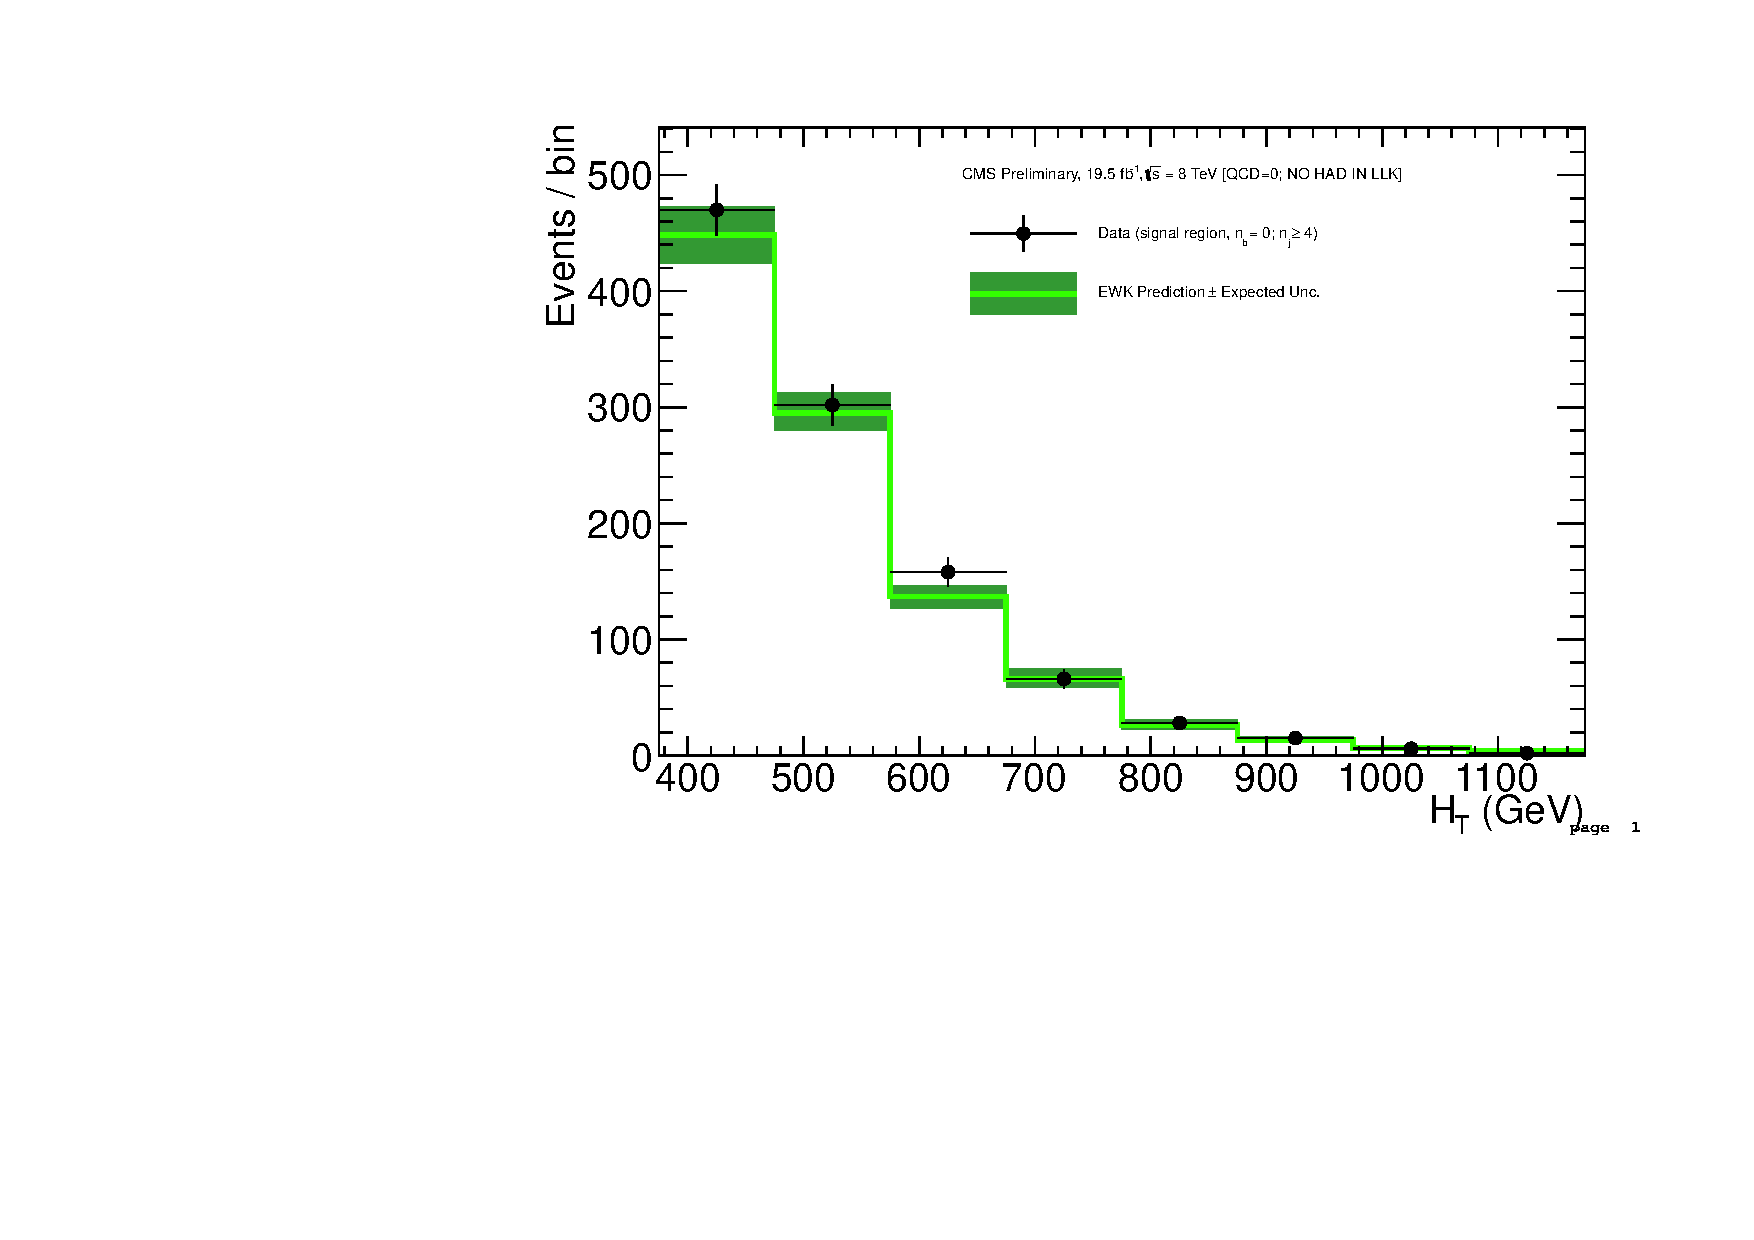
\includegraphics[width=0.45\textwidth,page=1]{figures/fit/v21/bestFit_2012pf_RQcdZero_fZinvAll_0b_ge4j-1p_smOnly}
    } 
    \subfigure[Hadronic sample (logarithmic scale)]{
      \includegraphics[width=0.45\textwidth,page=2]{figures/fit/v21/bestFit_2012pf_RQcdZero_fZinvAll_0b_ge4j-1p_smOnly}
    } \\
    \subfigure[$\mu$ + jets sample]{
      \includegraphics[width=0.45\textwidth,page=4]{figures/fit/v21/bestFit_2012pf_RQcdZero_fZinvAll_0b_ge4j-1p_smOnly}
    } 
    \subfigure[$\gamma$ + jets sample]{
      \includegraphics[width=0.45\textwidth,page=6]{figures/fit/v21/bestFit_2012pf_RQcdZero_fZinvAll_0b_ge4j-1p_smOnly}
    } 
    \caption{\label{fig:best-fit-control-only-ge4j0b} Comparison of the
      \scalht-binned observed data yields and SM expectations when
      requiring \njethigh and $\nb = 0$ for the (a-b) hadronic, (c)
      \mj, (d) \mmj and (e) \gj samples, as determined by a
      simultaneous fit to the data control samples only. The observed
      event yields in data (black dots) and the expectations and their
      uncertainties (dark green solid line with light green bands), as
      determined by the simultaneous fit, are shown. }
%      For illustrative purposes only, the signal expectations (pink
%      dashed line) for the model \texttt{T2cc} with $m_{\sq} =
%      250\GeV$ and $m_{\text{LSP}} = 170\GeV$ are stacked on top of
%      the SM expectations.}
  \end{center}
\end{figure}

\clearpage
\begin{figure}[t!]
  \begin{center}
    \subfigure[Hadronic sample (linear scale)]{
      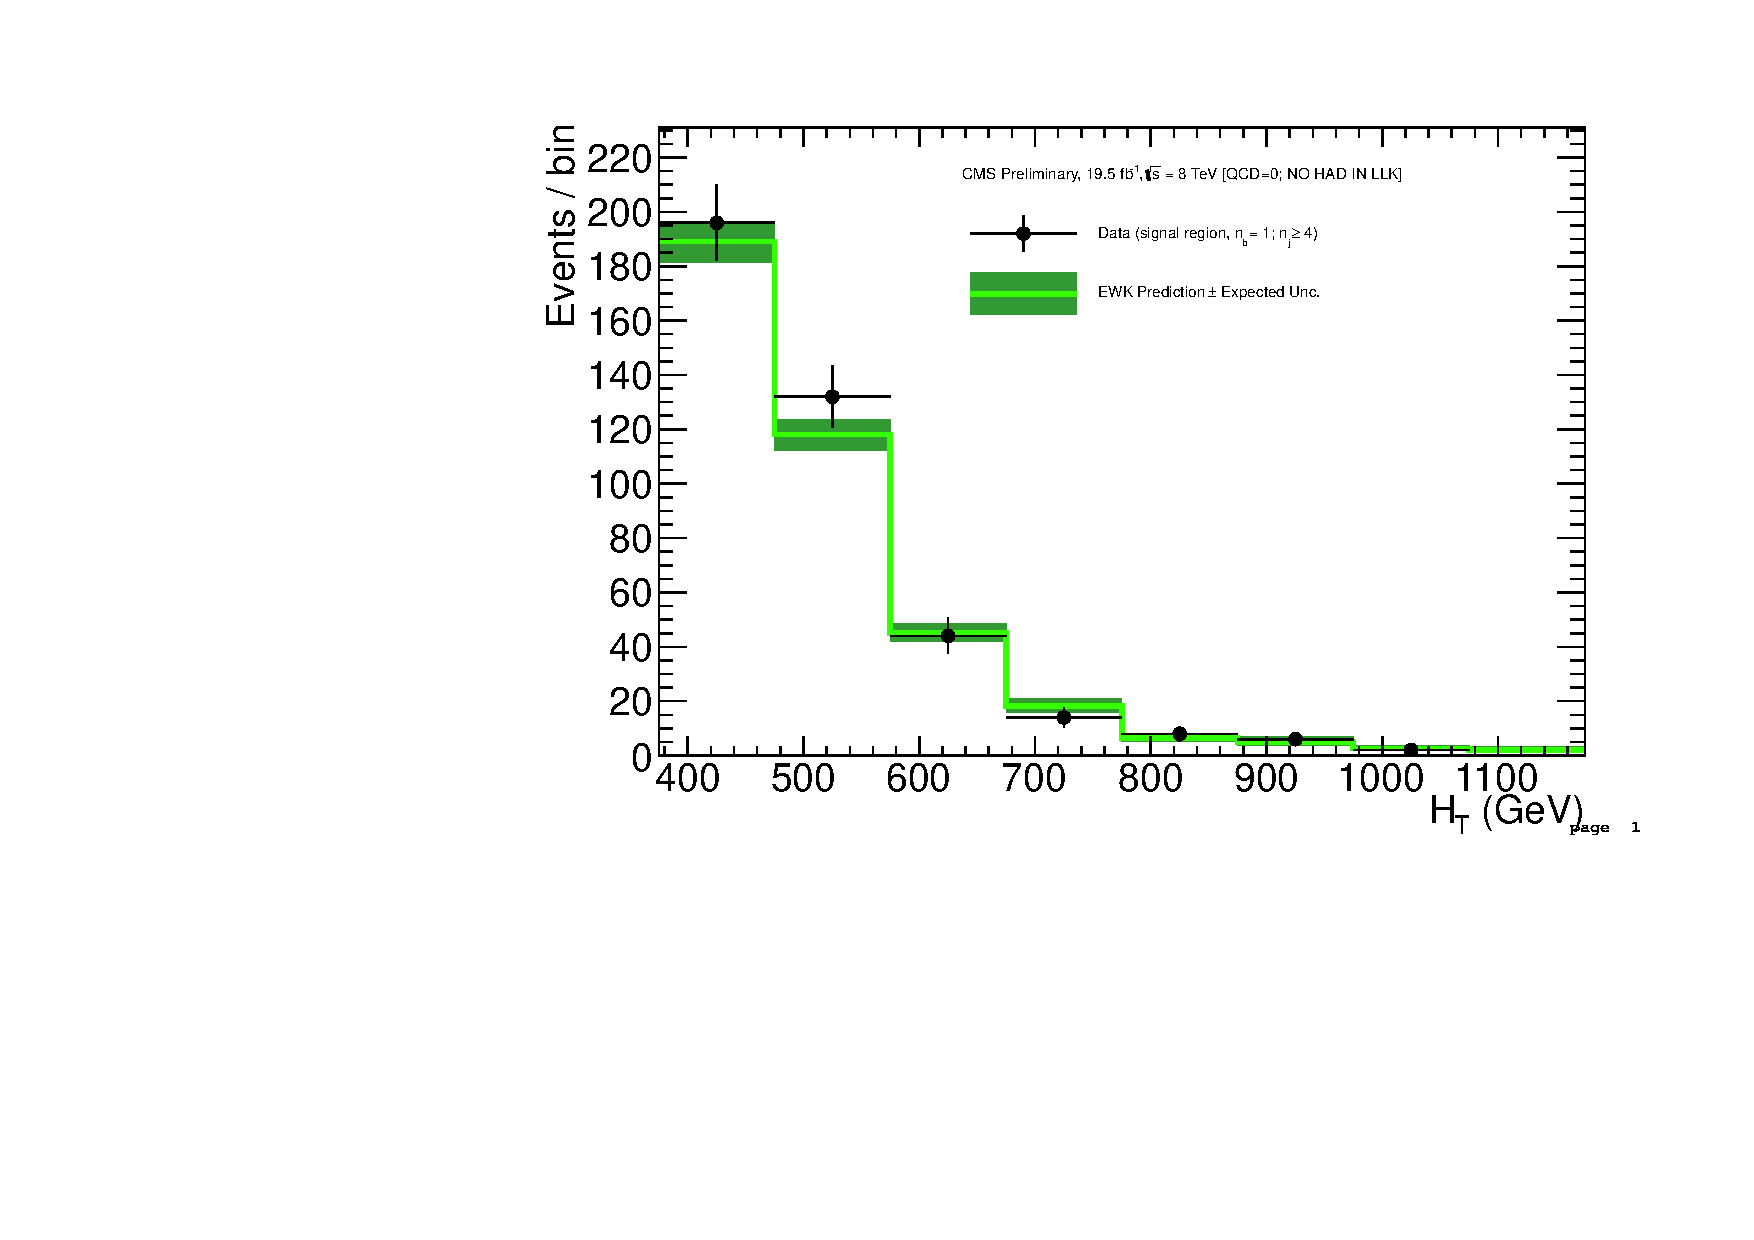
\includegraphics[width=0.45\textwidth,page=1]{figures/fit/v21/bestFit_2012pf_RQcdZero_fZinvAll_1b_ge4j-1p_smOnly}
    } 
    \subfigure[Hadronic sample (logarithmic scale)]{
      \includegraphics[width=0.45\textwidth,page=2]{figures/fit/v21/bestFit_2012pf_RQcdZero_fZinvAll_1b_ge4j-1p_smOnly}
    } \\
    \subfigure[$\mu$ + jets sample]{
      \includegraphics[width=0.45\textwidth,page=4]{figures/fit/v21/bestFit_2012pf_RQcdZero_fZinvAll_1b_ge4j-1p_smOnly}
    } 
    \subfigure[$\gamma$ + jets sample]{
      \includegraphics[width=0.45\textwidth,page=6]{figures/fit/v21/bestFit_2012pf_RQcdZero_fZinvAll_1b_ge4j-1p_smOnly}
    } 
    \caption{\label{fig:best-fit-control-only-ge4j1b} Comparison of the
      \scalht-binned observed data yields and SM expectations when
      requiring \njethigh and $\nb = 1$ for the (a-b) hadronic, (c)
      \mj, (d) \mmj and (e) \gj samples, as determined by a
      simultaneous fit to the data control samples only. The observed
      event yields in data (black dots) and the expectations and their
      uncertainties (dark green solid line with light green bands), as
      determined by the simultaneous fit, are shown. }
%      For illustrative purposes only, the signal expectations (pink
%      dashed line) for the model \texttt{T2cc} with $m_{\sq} =
%      250\GeV$ and $m_{\text{LSP}} = 170\GeV$ are stacked on top of
%      the SM expectations.}
  \end{center}
\end{figure}

\clearpage
\begin{figure}[t!]
  \begin{center}
    \subfigure[Hadronic sample (linear scale)]{
      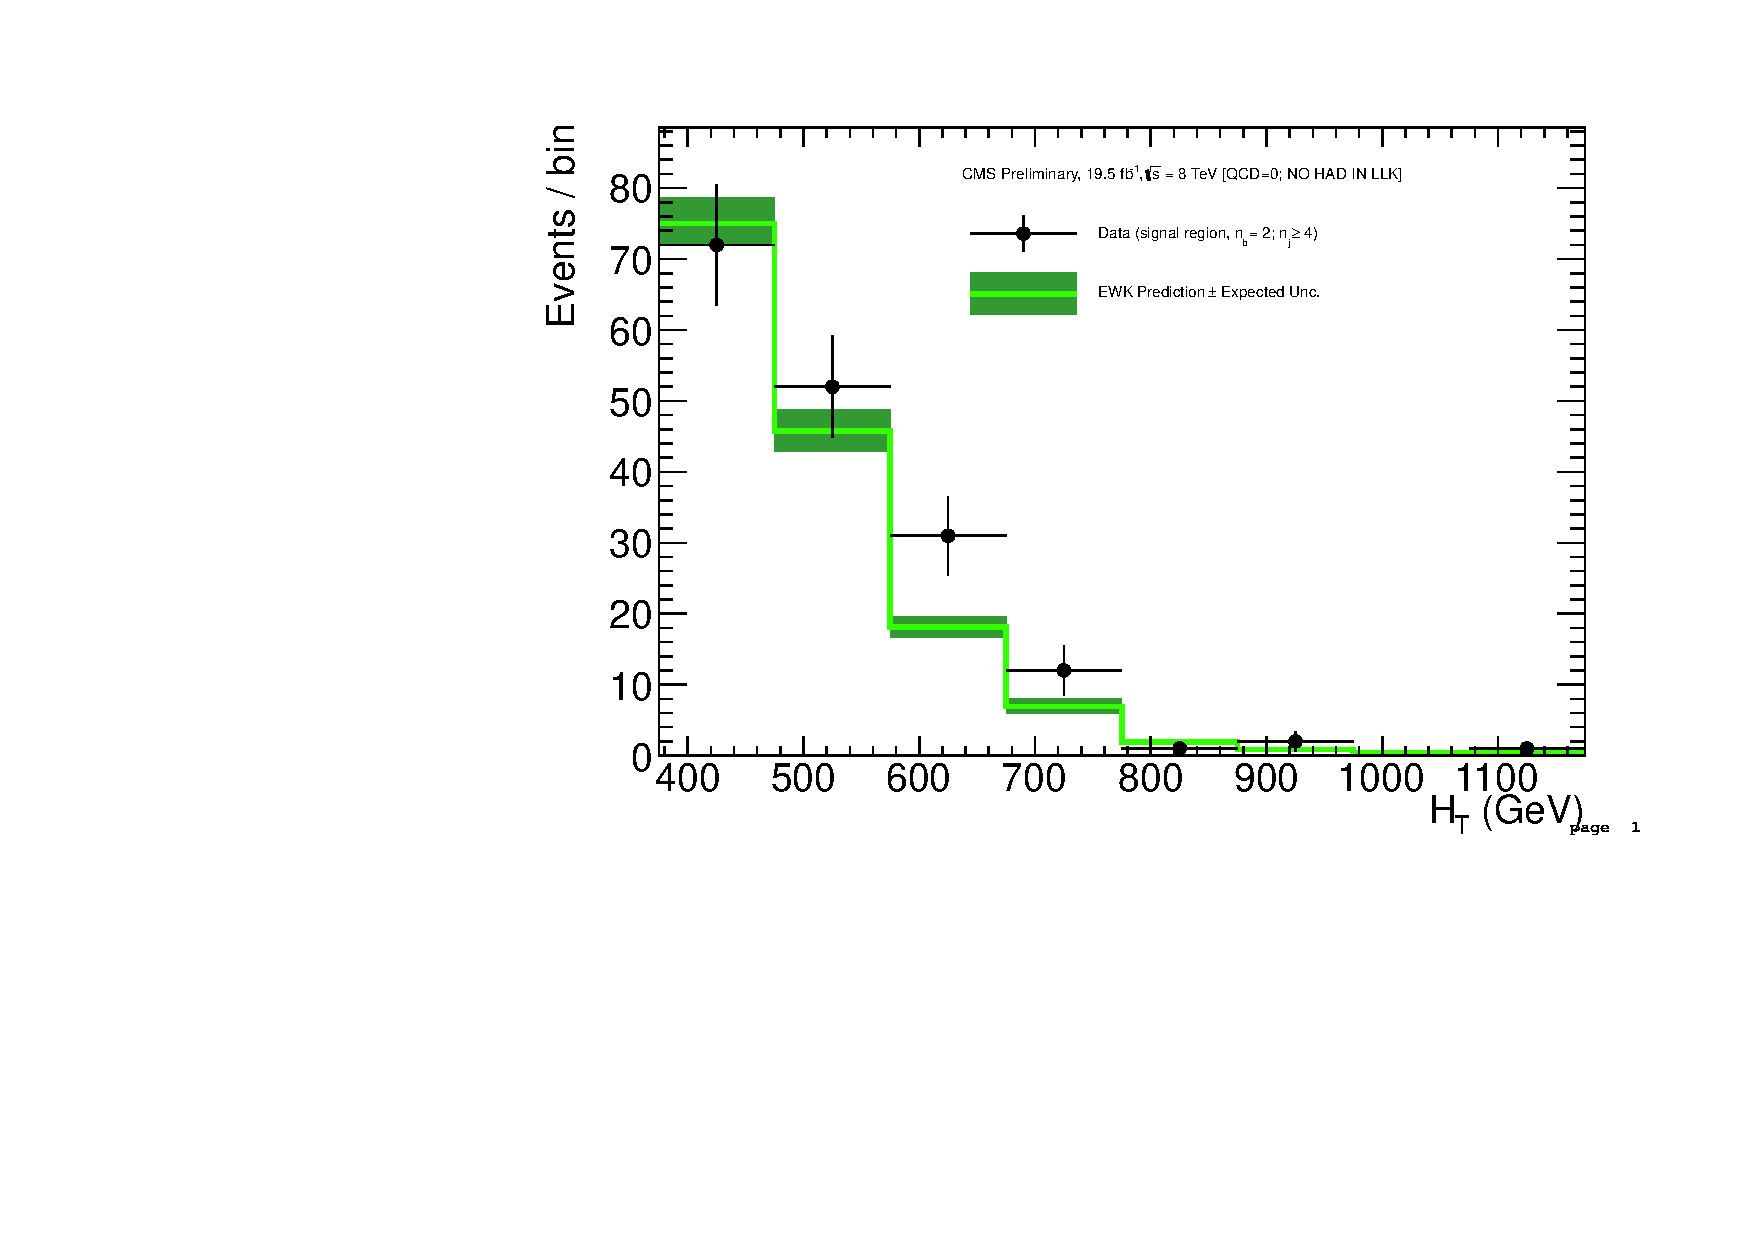
\includegraphics[width=0.45\textwidth,page=1]{figures/fit/v21/bestFit_2012pf_RQcdZero_fZinvAll_2b_ge4j-1_smOnly}
    } 
    \subfigure[Hadronic sample (logarithmic scale)]{
      \includegraphics[width=0.45\textwidth,page=2]{figures/fit/v21/bestFit_2012pf_RQcdZero_fZinvAll_2b_ge4j-1_smOnly}
    } \\
    \subfigure[$\mu$ + jets sample]{
      \includegraphics[width=0.45\textwidth,page=4]{figures/fit/v21/bestFit_2012pf_RQcdZero_fZinvAll_2b_ge4j-1_smOnly}
    } 
    \caption{\label{fig:best-fit-control-only-ge4j2b} Comparison of the
      \scalht-binned observed data yields and SM expectations when
      requiring \njethigh and $\nb = 2$ for the (a-b) hadronic, (c)
      \mj, (d) \mmj and (e) \gj samples, as determined by the \mj data
      control sample only. The observed event yields in data (black
      dots) and the expectations and their uncertainties (dark green
      solid line with light green bands) are shown. }
%      For illustrative purposes only, the signal expectations (pink
%      dashed line) for the model \texttt{T2cc} with $m_{\sq} =
%      250\GeV$ and $m_{\text{LSP}} = 240\GeV$ are stacked on top of
%      the SM expectations.}
  \end{center}
\end{figure}


%\clearpage
%\begin{figure}[t!]
%  \begin{center}
%    \subfigure[Hadronic sample (linear scale)]{
%      \includegraphics[width=0.45\textwidth,page=1]{figures/fit/v21/bestFit_2012pf_RQcdZero_fZinvAll_3b_ge4j-1_smOnly}
%    } 
%    \subfigure[Hadronic sample (logarithmic scale)]{
%      \includegraphics[width=0.45\textwidth,page=2]{figures/fit/v21/bestFit_2012pf_RQcdZero_fZinvAll_3b_ge4j-1_smOnly}
%    } \\
%    \subfigure[$\mu$ + jets sample]{
%      \includegraphics[width=0.45\textwidth,page=4]{figures/fit/v21/bestFit_2012pf_RQcdZero_fZinvAll_3b_ge4j-1_smOnly}
%    } 
%    \caption{\label{fig:best-fit-control-only-ge4j3b} Comparison of the
%      \scalht-binned observed data yields and SM expectations when
%      requiring \njethigh and $\nb = 3$ for the (a-b) hadronic, (c)
%      \mj, (d) \mmj and (e) \gj samples, as determined by the \mj data
%      control sample only. The observed event yields in data (black
%      dots) and the expectations and their uncertainties (dark green
%      solid line with light green bands) are shown. }
%%      For illustrative purposes only, the signal expectations (pink
%%      dashed line) for the model \texttt{T2cc} with $m_{\sq} =
%%      250\GeV$ and $m_{\text{LSP}} = 240\GeV$ are stacked on top of
%%      the SM expectations.}
%  \end{center}
%\end{figure}
%
%
%\clearpage
%\begin{figure}[t!]
%  \begin{center}
%    \subfigure[Hadronic sample (linear scale)]{
%      \includegraphics[width=0.45\textwidth,page=1]{figures/fit/v21/bestFit_2012pf_RQcdZero_fZinvAll_ge4b_ge4j-1_smOnly}
%    } 
%    \subfigure[Hadronic sample (logarithmic scale)]{
%      \includegraphics[width=0.45\textwidth,page=2]{figures/fit/v21/bestFit_2012pf_RQcdZero_fZinvAll_ge4b_ge4j-1_smOnly}
%    } \\
%    \subfigure[$\mu$ + jets sample]{
%      \includegraphics[width=0.45\textwidth,page=4]{figures/fit/v21/bestFit_2012pf_RQcdZero_fZinvAll_ge4b_ge4j-1_smOnly}
%    } 
%    \caption{\label{fig:best-fit-control-only-ge4jge4b} Comparison of the
%      \scalht-binned observed data yields and SM expectations when
%      requiring \njethigh and $\nb \geq 4$ for the (a-b) hadronic, (c)
%      \mj, (d) \mmj and (e) \gj samples, as determined by the \mj data
%      control sample only. The observed event yields in data (black
%      dots) and the expectations and their uncertainties (dark green
%      solid line with light green bands) are shown. }
%%      For illustrative purposes only, the signal expectations (pink
%%      dashed line) for the model \texttt{T2cc} with $m_{\sq} =
%%      250\GeV$ and $m_{\text{LSP}} = 240\GeV$ are stacked on top of
%%      the SM expectations.}
%  \end{center}
%\end{figure}
